\documentclass[]{article}
\usepackage{mathtools}
\usepackage{graphicx}
\usepackage{hyperref}

%opening
\title{Visualizing Graduate Admissions Data \\ CMPS 161: Final Project}
\author{Aaron Doubek-Kraft \\ adoubekk@ucsc.edu}
\date{March 20, 2017}



\begin{document}
	
\begin{titlepage}

	\maketitle

	\begin{abstract}
		Abstract goes here!
	\end{abstract}

\end{titlepage}

\section{Introduction}

	\indent \indent In 2017, there were nearly 1100 applicants to the UC Santa Cruz Computer Science graduate program. Given the unusually large size of this applicant pool, making sense of any large-scale trends simply by looking at their records in a table becomes an intractable problem. In addition to the high volume of applicants, the students' records contain a large number of potentially significant variables to be analyzed. This includes quantitative data, such as test scores and GPA, and qualitative data, such as the applicants' research interests, countries of origin, and whether or not the student was admitted.  In this paper, I attempt to develop visualizations to identify correlations in this data that could be relevant to the selection process. I have attempted to make this paper accessible to a reader with no background in visualization by providing high-level explanations alongside technical descriptions of the problem and my approach.

\section{Methods}

	\indent \indent The large number of variables and the high volume of records to be analyzed makes this a classic multivariate visualization problem, and so I take a relatively standard approach: the parallel coordinate plot. In a typical graph, the number of variables available to be displayed is limited to two or three, the number of spatial dimensions, so only correlations between a relatively small number of variables may be analyzed at a time (for example, in a scatter plot). The parallel coordinate plot generalizes the graphical approach to an arbitrary number of axes, allowing correlations to be analyzed across a large number of variables.

	\begin{figure}[h]
		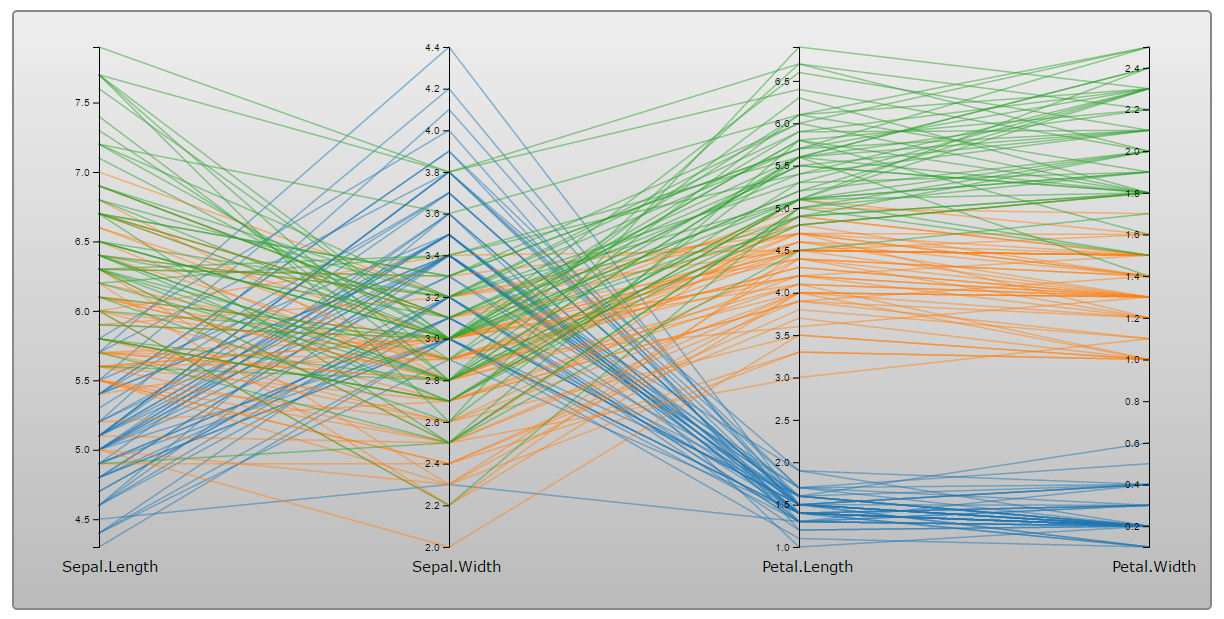
\includegraphics[width=\linewidth]{iris.png}
		\caption{Visualizing Edgar Anderson's Iris dataset. In this example, color is mapped to species of iris.}
		\label{fig:Result}
	\end{figure}
	
	\par As an example, I present a standard test case for multivariate visualization: the iris dataset.\cite{datasets} Even in the absence of any specific knowledge about irises, some trends are immediately apparent. First, petal length and petal width are clustered for a given species, and they appear to be directly correlated: irises either have large petals or small petals. Similarly, sepal length and sepal width are also clustered, though not as strongly as petal size, and they appear to be inversely correlated (in case the reader is curious, the sepals are the green parts outside the flower that protect the petals, a fact I had to look up). Using the high dimensionality, we can compare axes across the chart, and we can see that sepal length is also correlated to petal width. Now, the strength of this approach becomes clear: it would have taken four or five lower-dimensional charts such as scatterplots to reach the same conclusions that are presented here in one condensed figure. I leave analyzing the significance of these trends to the botanists.
	
	\par The parallel coordinate plot, in its most basic form, also has the advantage of simplicity: straight lines connecting parallel axes are not difficult to implement, especially given the powerful scaling and rendering functionality of the d3.js library\cite{d3} used in this project. The challenge is in scaling the visualization up to larger datasets. The iris dataset consists of only 150 records, while the graduate admissions data has almost 1100, so approximately seven times the number of lines will be drawn on the plot. Without some additional adjustments, the plot will be too visually cluttered to be of any use. One simple technique to improve readability is to map the color of the lines to their group membership, as color is mapped to species in the iris example. I will discuss additional techniques in the Implementation section.
\section{Implementation}
	\subsection{Dataset: Description and Processing}
		The dataset consists of 1097 records, each representing an applicant to one of the UCSC computer science graduate programs. The fields are described as follows:
		
		\begin{tabular}{c|c}
		 Field & Description \\ \hline
		 ID & Applicant identification number \\
		 Tags & Filters and Professors' interest in applicant\\
		 Transcripts Rec'd & Number of transcripts received \\ 
		 Transcripts Req'd & Number of transcripts required \\
		 Letters Rec'd & Number of recommendation letters received\\
		 Dept & Academic Department (all CMPS)\\
		 Degree & Masters or PHD\\
		 Research Interests & Applicant's list of research interests\\
		 Schools Attended & Applicant's previous education\\
		 UG GPA & Undergraduate GPA\\
		 UG GPA SCALE & Scale for undergraduate GPA\\ 
		 UG GPA (Normalized) & Defined as $\frac{GPA}{Scale}$\\ 
		 GRAD GPA & Graduate GPA\\
		 GRAD GPA SCALE & Scale for graduate GPA\\
		 GRAD GPA (Normalized) &  Defined as $\frac{GPA}{Scale}$\\
		 GREV & GRE - Verbal Reasoning\\
		 GREV\% & Percentage of total possible GREV score\\
		 GREQ & GRE - Quantitative Reasoning\\
		 GREQ\% & Percentage for GREQ\\
		 GREA & GRE - Analytical Writing\\
		 GREA\% & Percentage for GREA\\
		 GRESubjName & GRE Subject Test Name \\ 
		 GRESubjScore & Gre Subject Test Score\\
		 GRESubj\% & Gre Subject Test Percentage\\
		 TOEFL & Test Of English as a Foreign Language\\
		 IELTS & International English Language Testing System \\
		 Gender & Male, Female, Other, or Unreported\\
		 Ethnicity & \\
		 CA Res & California Resident: Yes, No, or Unreported\\
		 For/Dom & Domestic, or Country of Origin\\
		 Number of Reviews & \\ 
		 Ratings & \\ 
		 Avg. Rating & \\ 
		 Admitted & Yes or No\\
		\end{tabular} \\
		
		\par Since the applicants come from all around the world (in fact, the vast majority of applicants were foreign), one obstacle to drawing objective quantitative comparisons between groups of students was the fact that not all students have taken the same tests, and GPA is scaled differently in different countries. Normalizing the GPAs was relatively straightforward, since the dataset includes both the student's GPA and the GPA scale used, so the scores were simply normalized to 1, or in other words, the fraction of the appropriate total possible GPA. Additionally, a small number of the reported GRE scores were far higher the actual maximum score on the exam\cite{GRE}, so these were simply thrown out.
	\subsection{Developing Visualization}
		\par In this section, I will discuss the strategies implemented in this project to improve readability of parallel coordinate plots of large datasets. While the primary objective here was analysis of the graduate admissions data, the techniques used here, and in fact the interface itself, could be used to visualize any multivariate dataset stored as a csv file. In general, however, csv is a relatively loose standard\cite{csv}, so any truly generic application is nearly impossible.
		\subsubsection{Color Mapping}
			As the interface was designed to be a relatively generic approach to multivariate data, the program will parse potential relevant groups from the dataset itself and color-code them according to group membership. If the dataset contains multiple potential groupings, as the graduate admissions data does, the interface also allows the user to decide which grouping to use. This facilitates comparisons between subsets of the data, as well as identifications of correlations within a particular group.
		\subsubsection{Highlighting}
			If the user is interested only in a certain subset or subsets of the data, those may be selected, and all other subsets will be grayed out. This further emphasizes correlations (or the lack thereof) within this subset.
		\subsubsection{Brushing}
			Brushing involves selecting only those records which fall in a particular range on a given axis \cite{bostock,kosara}, and highlighting the associated polylines. This technique is particularly well suited to identifying correlations in larger datasets, because it allows the user to identify clusters within the data, and track those clusters across the many variables.
			\begin{figure}[h]
				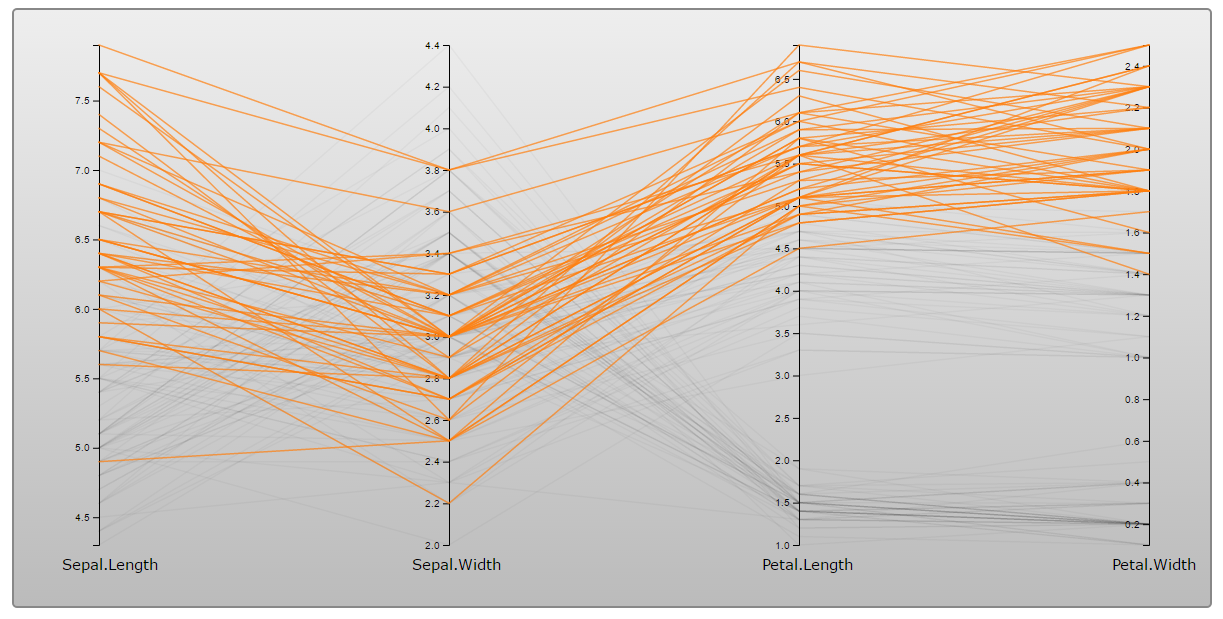
\includegraphics[width=\linewidth/2]{highlight.png}
				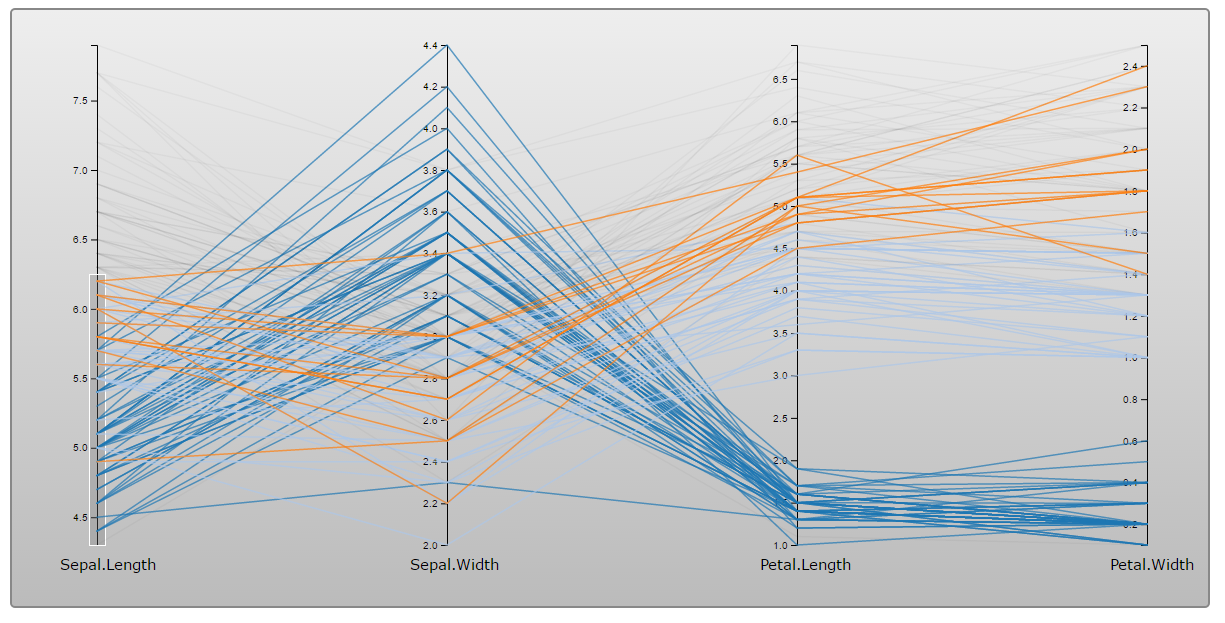
\includegraphics[width=\linewidth/2]{brush.png}
				\caption{Left: Iris dataset, with only species \textit{setosa} highlighted. Right: same dataset, with a brush applied for low sepal width.}
				\label{fig:Brush/Highlight}
			\end{figure}
		\subsubsection{Axis Selection}
		The visualization interface allows the user to select what axes to be displayed on the plot. While most of the strategies discusses here focus on highlighting clusters or trends in the data, this was implemented as a way to reduce the scale of the problem. For example, variables that take on only a small range of discrete values are typically not suited to this type of visualization\cite{kosara}, so this tool can simply eliminate such variables from the view.
		\begin{figure}[h]
			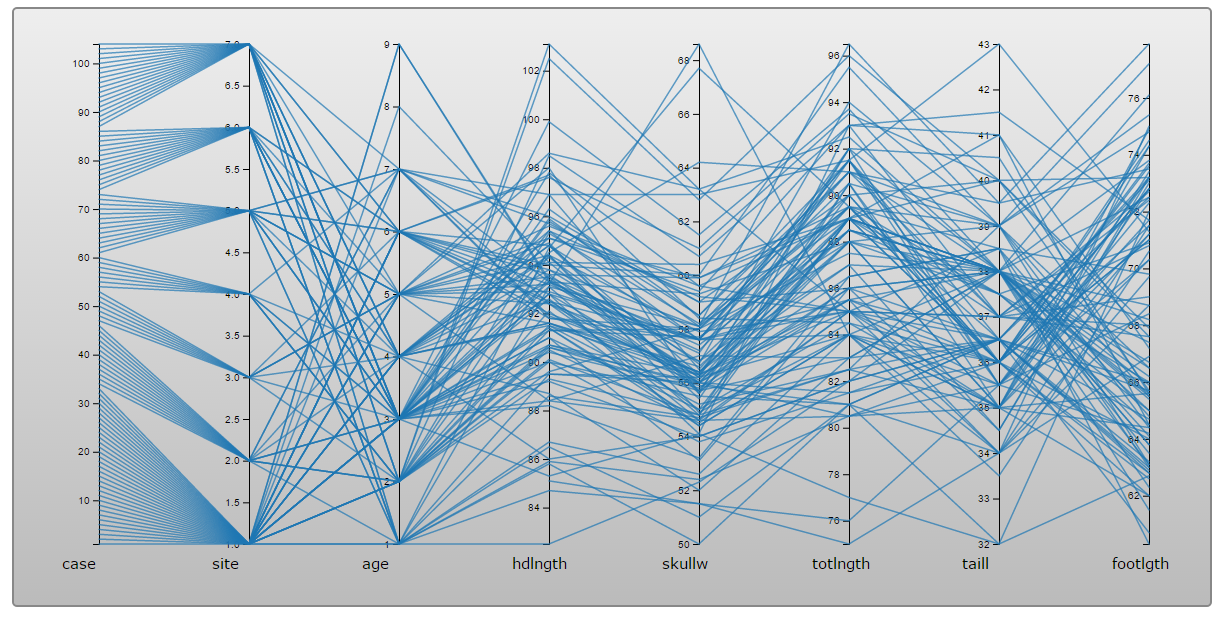
\includegraphics[width=\linewidth/2]{possum_bad.png}
			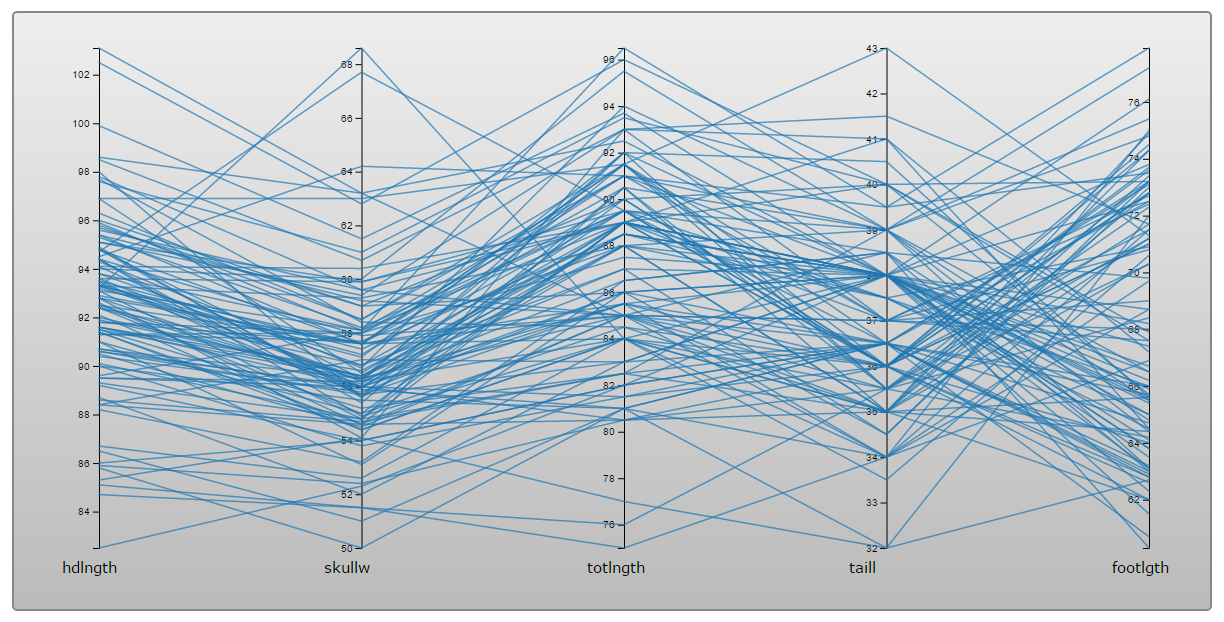
\includegraphics[width=\linewidth/2]{possum_good.png}
			\caption{Left: Possum dataset\cite{datasets}, with axes on left side taking on discrete values. Right: same dataset, with discrete axes eliminated using axis selection.}
			\label{fig:Axis}
		\end{figure}
	\subsection{Technical}
		This project uses d3.js to handle the rendering of the visualizations, jQuery.js for DOM manipulation and user input, w3.css as a style framework, and Python scripts for dataset processing tasks.
\section{Results}

\section{Conclusion}

\begin{thebibliography}{11}
	\bibitem{bostock}
		Bostock, Mike. Parallel Coordinates Example [Internet]. d3.js; Available from \url{http://mbostock.github.io/d3/talk/20111116/iris-parallel.html}
	\bibitem{csv}
		Comma Separated Values (CSV) Standard File Format [Internet]. Edoceo. Available from \url{http://edoceo.com/utilitas/csv-file-format}
	\bibitem{d3}
		d3.js: Data Driven Documents. Available from \url{https://d3js.org/}
	\bibitem{GRE}
		GRE Scores [Internet]. Available from \url{https://www.ets.org/gre/revised_general/scores/?WT.ac=grehome_grescores_150213}
	\bibitem{kosara}
		Kosara, Robert. Parallel Coordinates [Internet]. Eagereyes; 2010. Available from \url{https://eagereyes.org/techniques/parallel-coordinates}
	\bibitem{datasets}
		R Datasets [Internet]. Available from: \url{https://vincentarelbundock.github.io/Rdatasets/datasets.html}
	\bibitem{telea}
		Telea, Alexandru C. Data Visualization Principles and Practice. 2nd Edition. Boca Raton(FL): CRC Press; 2015.


\end{thebibliography}


\end{document}